\chapter{Methods} \label{chapter:MD}

\lettrine{M}{olecular Dynamics} simulations have been rightly defined as the `Computational Microscope' \citep{Lee2009,Dror2012} as they offer otherwise inaccessible insights into the molecular details underlying conformational changes of proteins and nucleic acids. Computational methods and tools based on MD are routinely applied in structural biology to quantitatively characterise the dynamics and thermodynamics of proteins and their complexes. MD simulations and the associated force fields are commonly used in the process of structure determination from NMR data or in theoretical structure prediction from homology models \citep{Vogel2017,Heo2018}. In particular, simulations of the structure help in relieving the artefacts deriving from the experiments, or in determining the correct conformation in cases when the experimental measure or the homology modelling has a large uncertainty.

Modelling and simulating a biological system consists in describing its components and their mutual interactions, by implementing the laws of physics in the attempt to reproduce the dynamics of phenomena observed in nature. A quantum mechanics description would be the most accurate, but it is computationally too expensive to achieve for large systems. To facilitate the task, several simplified models have been devised, each suitable to investigate particular cases.
%
In particular, a popular approach is a classical mechanics description of the dynamics (classical : quantum mechanics effects are relevant on very short time and length scales only. Therefore, for systems of biological relevance (at the microsecond time scale and nanometer length scale) the classical approximation is sufficiently accurate, and a model computationally affordable.

Another computational method for tackling similar problems is to adopt a probabilistic approach rather than MD: instead of using the laws of mechanics to evolve the system, a random sampling of its states is performed to find the most energetically favoured ones. This procedure, the Monte Carlo (MC) method, partially relieves the computational burden with respect to a dynamic approach, as it does not need to compute the forces acting on the particles, but only the energy of the system. MC simulations have been successfully used in situations where the system can get trapped in an energy minimum if simulated through MD, while it is deemed that many more minima are present, and thus a more extensive sampling is sought \citep{Liu2012}. However, MC does not capture dynamical properties and thus can be unsuitable for some questions posed on biological systems.
%
Despite the focus of the present work is Molecular Dynamics, it is important to be aware of alternative computational techniques as a complementary tool which can boost the understanding of the system.

We briefly present here the core theory and implementation of classical MD simulations, especially discussing the parametrisation of the different force fields used in this work, as a consistent part of it focuses on testing and implementing MD simulations parameters. Understanding their methodology provides an interpretative key with which simulations must be designed, run and interpreted in each specific case \citep{vanGunsteren2006}. We will also discuss the strengths and limitations of MD simulations and their comparison with experiments. A review of relevant successes of MD simulations will complete the chapter.


\section{Algorithms for Molecular Dynamics: the Newton's law} \label{sec:md_algos}
In a classical MD framework, Newton's second law of motion rules the dynamics, stating that the acceleration $\textbf{a}$ that a particle is subject to at time $t$, depends on the total force $\textbf{F}$ acting on the particle itself and on its mass $m$ (bold denotes vectorial quantities):
\begin{equation} \label{eq:newton}
\textbf{F}(t) =  m \cdot \textbf{a}(t) \, .
\end{equation}
As the acceleration $\textbf{a}(t)$ is the second derivative of the position $\textbf{r}(t)$ with respect to time, given the initial position and velocity of the particle ($\textbf{r}(t_0)$, $\textbf{v}(t_0)$), their temporal evolution can be computed integrating $\textbf{a}(t) = \textbf{F}(t)/m$ as follow:
\begin{eqnarray} \label{eq:analytical}
\mathbf{v}(t) &=& \mathbf{v}(t_0) + \int_{t_0}^t \frac{\mathbf{F}(t')}{m} \, dt' \, ; \\
\mathbf{r}(t) &=& \mathbf{r}(t_0) + \int_{t_0}^t \mathbf{v}(t') \, dt' + \int_{t_0}^t \int_{t_0}^{t'} \frac{\mathbf{F}(t')}{m} \, dt'' \, dt'\, .
\end{eqnarray}
In the case of complex biomolecular systems with many particles and multiple interactions acting between them, it is impossible to integrate analytically Equation \ref{eq:analytical}, while a different and feasible approach consists in discretising it.
%
The idea is to consider very short time steps of length $\Delta t$, so that in such intervals the forces are (almost) constant, and the integration of Equation \ref{eq:analytical} becomes trivial.
%
A careful choice of the values to integrate allows to reduce the approximations derived from such approach.
For example, choosing the velocity value at time $t_0 + \Delta t/2$ (and not at $t_0$) decreases the error down to orders of $(\Delta t)^4$ (rather than $(\Delta t)^2$). This framework is at the basis of the so-called leap-frog algorithm, which is used in the vast majority of MD engines:
\begin{eqnarray}
\mathbf{v}\left(t_0 + \frac{\Delta t}{2}\right) &=& \mathbf{v}\left(t - \frac{\Delta t}{2}\right) + \frac{\mathbf{F}(t)}{m} \, \Delta t \, ; \\
\mathbf{r}(t_0 + \Delta t) &=& \mathbf{r}(t_0) + \mathbf{v}\left(t_0 + \frac{\Delta t}{2}\right) \, \Delta t \, .
\end{eqnarray}
This algorithm can thus ``solve" every possible Newton equation, at the expenses of some precision.

\paragraph{Constraint algorithms} Considering that MD deals with bonded atoms belonging to multi-atoms molecules, the length of these bonds must be kept within a physically meaningful value. As the approximate procedure mentioned above may however give raise to unphysical configurations, constraint algorithms are applied after the update of atoms positions, to restrict the change in bond length. The ones used in this work are SETTLE \citep{Miyamoto1992} and LINCS (Linear Constraint Solver) \citep{Hess1997}: the first is an exact implementation of the solution for rigid bodies of three elements only (such as water molecules in their atomistic description), while the second finds an approximate solution for molecules with more atoms.

\paragraph{Thermostats and barostats} In addition to the constraint algorithms listed above, specific algorithms are needed to realistically reproduce the simulation's conditions of choice in terms of Temperature and Pressure.

In most cases, we are interested in simulating a system at constant temperature, which corresponds to a constant average kinetic energy $E_k$ (with the average performed over time).
%
Despite this condition seems less restrictive than imposing a constant $E_k$ at each time, the fluctuations from the average value must be distributed according to a specific statistics.

Statistical mechanics has investigated the problem identifying the possible states of a closed mechanical system in thermal equilibrium with a heat bath at a fixed temperature \citep{gibbs_2010}. This states form the so called \emph{canonical ensemble}, which can be completely defined knowing the number $N$ (and identity) of the particles, the temperature $T$, and the volume $V$ of the system itself.
%
Many other \emph{ensembles} are possible, according to the restrictions imposed on the system: for example, if the volume $V$ is allowed to vary but it is kept constant the pressure $P$ (a quantity we will define in the following paragraphs), we obtain the \emph{isothermal-isobaric ensemble}, defined by $N$, $P$ and $T$.
%
Again, a constant number $N$, volume $V$ and total energy $E$ define the \emph{microcanonical ensemble}.
%
These are the most common situations one wishes to reproduce in a Molecular Dynamics simulations, and thus effort has been directed to ensure their behaviour is reproduced at best in the simulations outcome. 
 

Regarding the situations at constant temperature, the approximations performed by the MD algorithm lead the kinetic energy to drift from its initial value. To ensure that temperature is maintained throughout the simulation, thermostat algorithms have been devised to rescale the velocities of selected particles.

The thermostats used in this work are the Berendsen \citep{Berendsen1984} and velocity rescale \citep{Bussi2007} ones.
They both rescale the velocities of all the particles in the simulation at each time step. For Berendsen, the rescaling factor $\lambda$ is computed imposing that the corrected kinetic energy $E^*_k$ is equal to:
\begin{equation} \label{eq:berend}
    E^*_k = \frac{1}{2} \left(\lambda v\right)^2  = \left( 1 - \frac{\Delta t}{\tau_T} \right) E_k + \frac{\Delta t}{\tau_T} E_k^0
\end{equation}
where $E_k^0$ is the target kinetic energy and $\tau_T$ is a time interval multiple of $\Delta t$ which regulates the strength of the coupling. A value of $\tau_T$ equal to $\Delta t$ would suppress all thermal fluctuations, while in real systems they are still allowed.
%
Even with larger $\tau_T$ though, this thermostat gives incorrect results as it can not maintain the correct distribution of velocities during the evolution of the dynamics, thus violating the statistics of the \emph{canonical ensemble}. To solve this problem, the velocity rescale thermostat was introduced \citep{Bussi2007}. It adds to the right side of Equation \ref{eq:berend} a stochastic term:
\begin{equation}
    2 \sqrt{\frac{E_k\,E_k^0}{\tau_T\,N_f}}\, dW
\end{equation}
with $N_f$ the number of degrees of freedom in the system and $dW$ a Wiener noise \citep{Durrett2010} which ensure fluctuations are sampled correctly.

The other relevant quantity, pressure, is defined as the average quantity of motion exchanged between the particles and the walls of the box they are confined to, which depends on their frequency of collision. Most MD simulations are run under periodic boundary conditions, i.e.\ a particle which exits from the simulation box during a move is brought back on the opposite side of the box. This mimics the presence of an infinite number of equivalent boxes one next to the other, and alleviates the finite size effects implicitly modelling an infinite simulation box.
%
As particles are not effectively bouncing on the walls, the pressure is computed from the velocities of the ones trespassing the box boundaries during a move.
%
Barostat algorithms rescale the size of the simulation box to adjust the collision frequency and thus the pressure to the target value.

As a note, pressure is an intensive quantity, i.e. a local physical property of a system and does not depend on the system size or the number of particles in it (extensive quantities). However, both these quantities are involved in its computation in the framework used. From the classic kinetic theory of gases, for a homogeneous gas of $N$ molecules of mass $m$ in a box of volume $V$, in isotropic conditions, the pressure can be computed as:
\begin{equation}
P = \frac{Nm\langle v^2\rangle}{3V}.
\end{equation}
Thus, rescaling the size of the system (extensive) and dividing $N$ (extensive) by this quantity, will influence the pressure (intensive).

Usually all the box dimensions are rescaled by the same amount. In the case of anisotropic systems like lipid simulations, an anisotropic coupling can be enforced: for these systems, the membrane patch is usually parallel to one side of the simulation box, and spans the whole side area. In this way, it joins with its periodic images, without any water molecules in between. This is convenient as it shields the hydrophobic core of the membrane from water, moreover it ensure that the membrane remains planar. Indeed, isolated patches of membrane tend to fold into vesicles to minimise their energy.
%
In the situation where the membrane joins its periodic images, to compute pressure, the box sides parallel to the membrane plane are rescaled separately with respect to the one perpendicular to it.
This is because lateral pressure exerted by the lipids is expected to be different with respect to the one of water.

The barostats used in this work are the Berendsen \citep{Berendsen1984} and Parrinello-Rahman \citep{Parrinello1981} ones. The Berendsen barostat is analogous to its thermostat counterpart, as it defines a scaling factor for the velocities (and thus the coordinates) based on the target and effective pressure $P_0$ and $P$, and a coupling time $\tau_P$:
\begin{equation} \label{eq:barostat_bere}
    v^* = v \left( 1 - \frac{\beta \, \Delta t \, (P_0 - P}{\tau_P} \right)^{1/3}
\end{equation}
where $\beta$ is the theoretical isothermal compressibility. As also the Berendsen barostat suffers from problems regarding the correct sampling of fluctuations, the Parrinello-Rahman is used for production runs. It introduces the constraint of constant pressure in the dynamical equations of the systems (in a Lagrangian approach) which allows to reproduce correctly the \emph{isobaric ensemble}.

It must be noticed that the use of the correct barostat is crucial when measuring, e.g., the true isothermal compressibility of the system $K$ (as opposed to the theoretical value $\beta$ introduced in Formula \ref{eq:barostat_bere}). This quantity is defined as the relative volume change as a response to a pressure change, and is directly related to the fluctuations of the volume at constant pressure:
\begin{equation}
K_T = \frac{\langle \Delta V \rangle ^2}{Vk_BT}.
\end{equation}
Clearly, an incorrect distribution of fluctuations would produce a wrong estimate of this quantity.

Finally, when choosing a thermostat and barostat to  be used in conjunction, one must check in the literature for their mutual compatibility to obtain the correct \emph{isothermal-isobaric ensemble}. For this reasons indeed, some pairings are not implemented in the standard MD engines.


\section{Force fields}

Force fields for classical MD simulations provide the expression of the potential energy of a system. Thus they determine the forces employed in Newton's law ruling the dynamics.
%
They usually rely on the breakdown of interactions into several independent, additive and derivable terms, identified on an empirical physical basis.

We report here the functional form of the GROMOS force field \citep{Oostenbrink2004,Schmid2011,Reif2012} implemented in the GROMACS MD simulation engine \citep{Berendsen1995,Abraham2015,gromacs_man}, as an example of a classical force field.
%
Other force fields can have slightly different implementations, however the general classification of interactions and the type of functional forms used are similar.

\paragraph{Covalent (bonded) interactions} Covalent interactions are modelled with potential energy terms representing bond stretching, angle bending, improper and proper dihedral angles torsion. 
%
The functional form of the potential energy function for each of them aims at a simplified, classical description of the atomic motion of molecules. Often, it is modelled as a harmonic-like vibration around the equilibrium position, regulated by a constant.
%
In the GROMOS force field, this translates in the equations displayed in Table \ref{table:ff}, where for proper dihedrals, the convention states that $\phi_{ijkl}$ is the angle between the ($i$, $j$, $k$) and ($j$, $k$, $l$) planes; with $i$, $j$, $k$, and $l$ four subsequent atoms, for example along a protein backbone. A value of zero for $\phi_{ijkl}$ corresponds to a \textit{cis} configuration (penalised) and $\pi$ to a \emph{trans} (favoured). The integer $n$ denotes the number of equally spaced energy minima available in a 360$^\circ$ turn.
%
The same conventions hold for improper dihedrals $\xi_{ijkl}$, which are used to ensure ring planarity and control the chirality of tetrahedric centres.

\begin{figure}[t]
\centering
 \def\arraystretch{1.6}
\begin{tabular}{lllll}
 \textbf{Type} & \multicolumn{2}{l}{\textbf{Eq. pos.}} & \textbf{Const.} & \textbf{Functional form} \\
 \hline
  Bond & b$_{ij}$ & k$^b_{ij}$ & $\frac{\text{kJ}}{\text{mol}\,\text{m}^2}$ & $V_b(\textbf{r}_{ij}) = \frac{1}{4}\,k^b_{ij}\,\left(|\textbf{r}_{ij}|^2 - b_{ij}^2\right)^2 $ \\ 
  Angle & $\theta^{\, 0}_{ijk}$ & $k^\theta_{ijk}$ & $\frac{\text{kJ}}{\text{mol}}$  & $V_a(\theta_{ijk}) = \frac{1}{2}\,k^\theta_{ijk}\,\left(\cos\left(\theta_{ijk}\right) - cos\left(\theta^{\, 0}_{ijk}\right)\right)^2$ \\
  Dihedral & $\phi_{ijkl}^{\, 0}$ & $k_{ijkl}^\phi$ & $\frac{\text{kJ}}{\text{mol}\,\text{rad}^2}$  & $V_d(\phi_{ijkl}) = k_{ijkl}^\phi\,\left( 1 + \cos\left( n \, \phi_{ijkl} - \phi_{ijkl}^{\, 0} \right) \right)$ \\
  Improper & $\xi_{ijkl}^{\, 0}$ & $k_{ijkl}^\xi$ & $\frac{\text{kJ}}{\text{mol}}$  & $V_{id} (\xi_{ijkl}) = \frac{1}{2}\,k_{ijkl}^\xi \left( \xi_{ijkl} - \xi_{ijkl}^{\, 0} \right)^2$ \\
  \hline
 \end{tabular}
\captionof{table}[Functional form of GROMOS force field]{Functional form of bonded interaction in the GROMOS force field implemented in GROMACS.}
\label{table:ff}
\end{figure}

It must be noticed that these types of potentials cannot model the rupture of a bond.


\paragraph{Non bonded interactions}
Non bonded interactions include the short range Pauli repulsion, the van der Waals attraction, and the long range electrostatic term.

The first two can be modelled together by a Lennard-Jones potential. Its functional form, describing the interaction between two neutral atoms at distance $r$, models the long range dispersion with a $r^{-6}$ behaviour typical of the dipole-dipole interactions found in noble gases (London dispersion forces), while the Pauli term is approximated by a $r^{-12}$ behaviour to ease the computation in relation with the previous one:
\begin{equation}
V_{LJ}(r) = 4 \epsilon \left[ \left( \frac{\sigma}{r} \right)^{12} - \left( \frac{\sigma}{r} \right)^6 \right].
\end{equation}
Two parameters, $\epsilon$ and $\sigma$, tune the interaction strength and the equilibrium distance. They are fitted against experimental data and are specific of each pair of atoms species.

The Coulomb energy between two charges $q_1$ and $q_2$ at distance $r$ is represented by the Coulomb law:
\begin{equation}
V_C(r) = \frac{1}{4 \pi \epsilon_0} \, \frac{q_i q_j}{\epsilon_r r_{ij}}
\end{equation}
with $\epsilon_0$ the dielectric constant of vacuum and $\epsilon_r$ the relative dielectric constant, introduced to properly take into account the screening provided by the material surrounding the object (usually water), as polarisability is not included in this description.

The treatment of non-bonded interactions requires particular care because of their long range nature: in every point of the simulation box many forces from distant atoms are acting at the same time, making the prediction of the outcome difficult.
%
The van der Waals forces decay fast, therefore the tail of their functional can be cut after a threshold distance with little impact on the outcome; while Coulomb interactions, with their slower decay, must be taken into account throughout the whole simulation box. Many algorithms have been devised to efficiently compute them, like the Particle Mesh Ewald \citep{Essmann1995} or the Reaction Field \citep{Tironi1995} approaches. 

Finally, all biomolecular force fields, and in particular their van der Waals interactions, are parametrised to describe systems at room temperature, therefore simulations performed at substantially different temperatures must be interpreted carefully.


\subsection{Classification of force fields} \label{sec:ff_ex}

\begin{figure}
\centering
\includegraphics[width=0.95\textwidth]{2methods/pics/picture_chapter}
%
\caption[Scheme of popular simulation force field for biomolecules]{List of popular simulation force field for biomolecules, ordered from detailed to coarse (reference to the relative papers in Section \ref{sec:ff_ex}). On the left, snapshot of notable systems simulated with the force fields CHARMM (adapted from \citet{Lipkin2017}); GROMOS (adapted from \citet{Macpherson2019}); SIRAH (adapted from \citet{Machado2017}) and MARTINI (adapted with permission from \citet{Samsudin2017}).}
\label{fig:ff}
\end{figure}

Many force fields for classical MD simulations adopt a functional form equal or similar to the one described above. Their difference lies in the number of degrees of freedom modelled, in a hierarchy of descriptions proceeding from detailed to coarse (Figure \ref{fig:ff}). Three possible classes of descriptions are:
\begin{itemize}
\item all-atoms force fields, where all the atoms are present in the description, and represented as spheres of variable size according to their van der Waals radius (e.g. proportional to $\sigma$ in a Lennard-Jones model). Examples of all-atoms force fields are AMBER \citep{Maier2015,Dickson2014,Wang2004_amber}, CHARMM \citep{MacKerell1998,Klauda2010,Huang2013} and OPLS all-atom \citep{Jorgensen1988}.
\item united-atoms force fields, similar to the previous ones but where non-polar hydrogens are incorporated in the heavy atom they are bonded to. The ``united" atom is given a new $\sigma$ parameter and increased mass according to how many hydrogen it includes. The GROMOS force field \citep{Oostenbrink2004,Schmid2011} follows this philosophy, and OPLS has also a united atom version \citep{Jorgensen1996}.
\item coarse-grained force fields, which group together in one unique bead few atoms, to reduce the number of variables to compute. The clustered atoms are such that their mutual distances are expected to vary little with respect to the ample movements of components of the system far away from each other (which will be grouped in different beads). The MARTINI \citep{Marrink2007,Monticelli2008,DeJong2013} and SIRAH \citep{Machado2018,Barrera2019} force fields belong to this category.
\end{itemize}
%
We now give a more detailed insight of the characteristics and parametrisation strategies of the atomistic and the coarse-grained force fields employed in this work.


\subsection{The GROMOS force field}
All-atom and united atom force fields are parametrised against first-principle or experimental values.
%
While for the all-atom force fields AMBER and CHARMM the parametrisation is based on \emph{ab initio} quantum mechanics calculations refined against experimental data \citep{Maier2015,Dickson2014,Wang2004_amber,MacKerell1998,Klauda2010}, the united-atom GROMOS force field relies on the reproduction of heat of vaporization of small molecules and free enthalpies of solvation of small compounds in different solvents, at physiological temperatures and pressures \citep{Oostenbrink2005,Schmid2011,Reif2013}.
%
These procedures sets not only the constants of the bonded interactions, but also the partial charges of the atoms inside a molecule: as no electrons are included for the sake of efficiency, their redistribution across atoms which are bonded is modelled through fractional charges assigned to each atom (while the total charge of a molecule must sum to an integer).
%
Moreover, it is assumed that the parametrisation performed for small moieties can be transferred to a larger compound including these moieties. This limits the number of chemical groups to be described in order to simulate biomolecules.

In every MD simulation, the description of water is crucial. Out of the many water model proposed, the GROMOS parametrisation has been performed with a flexible simple point charge (SPC \citep{Berendsen1981}) model. This description represents water as a three atoms molecule, with a negative charge on the oxygen and positive complementary charges on the two hydrogen atoms, and allows flexible hydrogen-oxygen bonds. This model reproduces correctly the density and dielectric permittivity of water \citep{Mark2001}. To be noticed that, from the point of view of the computation, water molecules are the vast majority of the particles involved in a simulation and thus a significant fraction of the computer time is spent in updating their positions and calculating solvent-solvent interactions.

The improvement of computational techniques and reparametrisation strategies prompts the periodical release of newer versions of force fields. In the present work, we employed version 53A6 of the GROMOS force field \citep{Oostenbrink2004} for the set of simulations involving peptidic assembly in solution, while we switched to 54A7 \citep{Schmid2011} and 54A8 \citep{Reif2013} for the simulations involving biological membranes. While it is advisable to always have a coherent set of parameters across simulations, to compare their outcome in a consistent manner, when extending the system simulated to include membranes, we deemed the newer parameter sets more suitable because of the improvements introduced in the phosphocholine head parametrisation \citep{Marzuoli2019} (see Chapter \ref{chapter:lip_par} for a complete discussion on lipid parametrisation in GROMOS).

\subsection{The SIRAH force field}

The first coarse-grained force field we introduce groups multiple atoms in one bead but aims at maintaining chemical and structural details of the biomolecules described. As such it sets itself between the atomistic GROMOS description, and the coarse-grained MARTINI force field \citep{Marrink2007,Monticelli2008,DeJong2013} which will be introduced in the following.

Two different approaches are taken to develop a coarse-grained force field: top-down and bottom-up. In the first, parameters are fitted directly to global quantities derived from experiments, as performed in the atomistic GROMOS parametrisation. In the second, coarse-grained simulations results are fitted to outcomes from atomistic ones.

SIRAH \citep{Darre2015,Machado2018,Barrera2019} is a top-down force field derived to fit structural properties of proteins. It aims at reducing the complexity of an atomistic description while still being able to reproduce the correct secondary structure of proteins across a wide variety of folds contained in the PDB, together with a correct representation of their dynamics.

To obtain this, it opts for a non-uniform granularity, i.e.\ according to the region of interest a different number of heavy atoms is grouped in a bead, from a minimum of two up to four. In the case of proteins, it maintains the backbone flexibility by grouping NH, C$_\alpha$H and CO in three different beads, while side chains are represented with less details, generally grouping three atoms together. A schematic of the mapping for each amino acid is shown in Figure \ref{fig:sirah}. Contrary to force fields where the amino acid backbone is mapped to one bead only, the SIRAH description allows to reproduce secondary structures without recurring to additional constraints.
%
The dual granularity approach is based on physico-chemical intuition, and is more difficult to generalise than a uniform one. Nevertheless, the force field has been recently extended to lipids \citep{Barrera2019}, while it comprised a parametrisation for DNA molecules since its infancy.
%
\begin{figure}[t!]
\centering
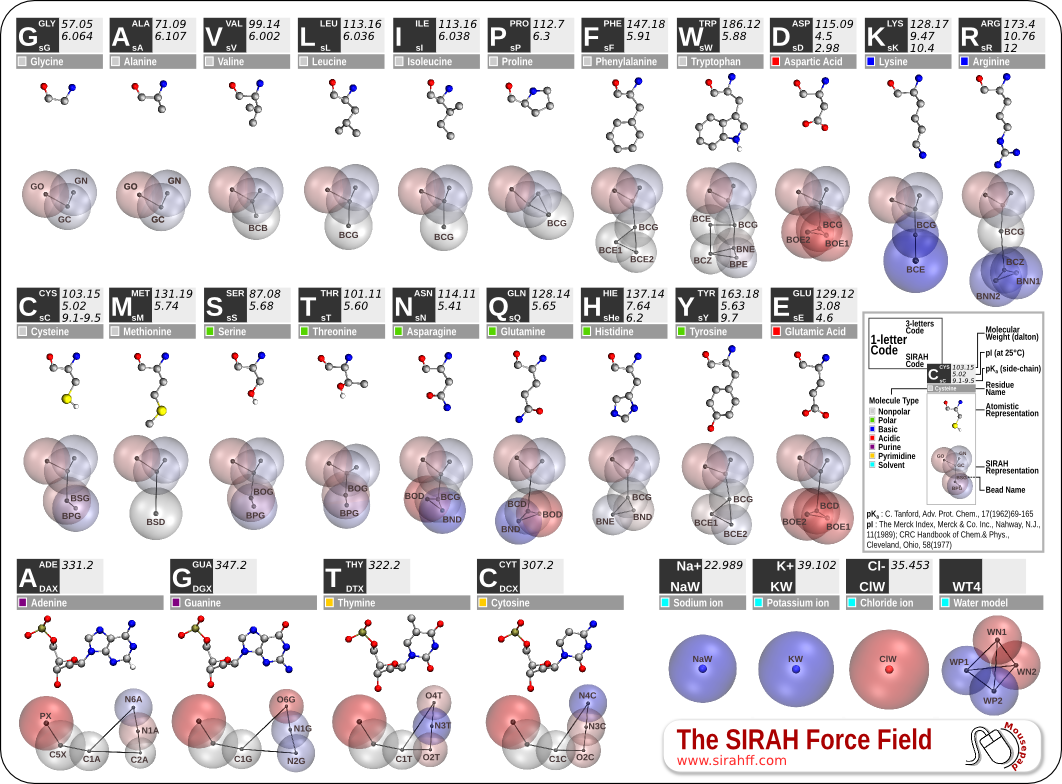
\includegraphics[width=0.8\linewidth]{2methods/pics/sirah_aa.png}
%
\caption[SIRAH force field amino acid and DNA description]{Description of amino acids and nucleic acids in the SIRAH force field. Reproduced from \citet{sirah_web}.}
\label{fig:sirah}
\end{figure}

The modelling of water in a coarse-grained force field is also critical: usually, a few water molecules are grouped together in one bead. This has two implications: water particles are large and thus cannot solvate very narrow pockets; moreover, collapsing the molecules in one single point in space removes the separation of charges, and the characteristic dipole every water molecule should have is lost. The dipole of water is responsible for hydrogen bonds formation and for the electrostatic screening observed in an aqueous solution. Such screening can be roughly modelled tuning the relative dielectric constant, but as this is a mean field approach, it cannot account for local effects.
%
To partially obviate to that, SIRAH force field maps four waters to a tetrahedral molecule, with one bead on each vertex: all the bonds are rigid, and the structure serves the purpose of having a repartition of plus and minus charges, by assigning a positive charge to two vertices and the opposite charge to the other two, giving a polarisable structure. The geometrical arrangement reproduces the tetrahedral network of water molecules observed in its liquid state, which is characteristic of this fluid and tunes its remarkable properties (as the high specific heat capacity, and the non-linear relationship between density and temperature in its liquid state). Finally, ions are represented as spheres including the ion and the first hydration shell comprising 6 water molecules.

Based on the above premises, SIRAH force field simulations of different peptides and proteins in solution proved to match the relative NMR results, showing a good reproduction of secondary structures; simulations of lipids randomly oriented in water showed the formation of an organised bilayer, and the expected behaviour of a few transmembrane proteins in model membranes was correctly reproduced \citep{Machado2018,Barrera2019}.

 
\subsection{The MARTINI force field}

The MARTINI force field is a popular coarse-grained description of biological molecules \citep{Marrink2007,Monticelli2008,DeJong2013}: developed originally with a focus on lipids, it has then been extended to include proteins, small ligands and DNA/RNA molecules \ref{fig:martini}.

MARTINI opts for a four-to-one approach, i.e.\ four heavy atoms are grouped in one bead. The number of bead types has been kept to the minimum necessary to represent biological molecules. They are organised systematically in polar, non-polar, apolar, or charged, and each type has a number of subtypes with increasing polarity to differentiate the chemical nature of the underlying atomistic structures.
%
This systematic approach can be easily transferred to new compounds, without the need of introducing new bead types.
%
The only exception is represented by rings molecules, where a two-to-one approach is needed to maintain the circular topology.

The MARTINI force field chooses a top-down approach to parametrise non-bonded interactions, tuning them against experimental partitioning free energies between polar and apolar phases, while bonded interactions are derived from reference all-atom information, in a bottom-up approach.

The four-to-one mapping implies that the amino acid backbone is represented by one bead only, preventing the description of directional bonds which are key to reproduce the secondary structure (Figure \ref{fig:martini_aa}). The bonded parameters partially account for this, favouring for each residue type the backbone conformation in which it is most likely found (as computed from the Protein Data Bank - PDB \citep{PDB}). When this is not sufficient, the protein can be constrained around a given structure through an elastic network model approach which constraints residues to keep their mutual position through harmonic potential applied on their backbone beads (ElNeDyn \citep{Periole2009}). However, both the backbone parametrisation and the use of ElNeDyn imply that local energy minima of the natural structure are not well sampled in MARTINI simulations, biasing the understanding of the structure dynamics.

The MARTINI force field provides two water models (Figure \ref{fig:martini_w}). The standard one groups four water molecules in one bead only, loosing the polarisability typical of water, the effect of which is partially restored with the use of a high dielectric constant. The polarisable water model \citep{Yesylevskyy2010} maps instead four water molecule to a single ``inflated" water, i.e.\ a three-beads molecule with the same shape of a single molecule, but expanded, and a charge splitting which can account for the water dipole.
%
\begin{figure}[t!]
\centering
\subbottom[]{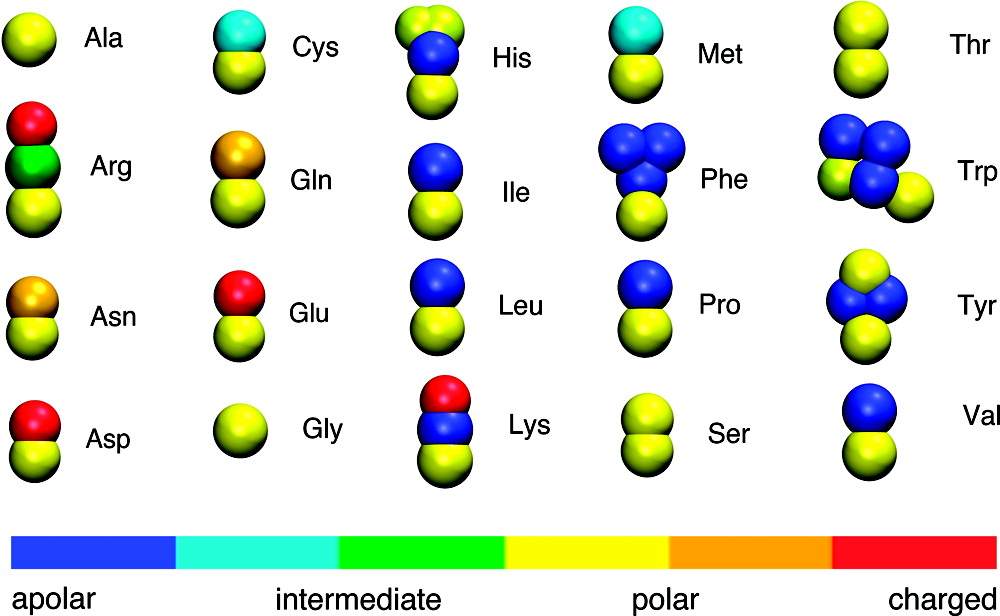
\includegraphics[width=0.7\linewidth]{2methods/pics/martini_aa.jpeg} \label{fig:martini_aa}} \\
\subbottom[]{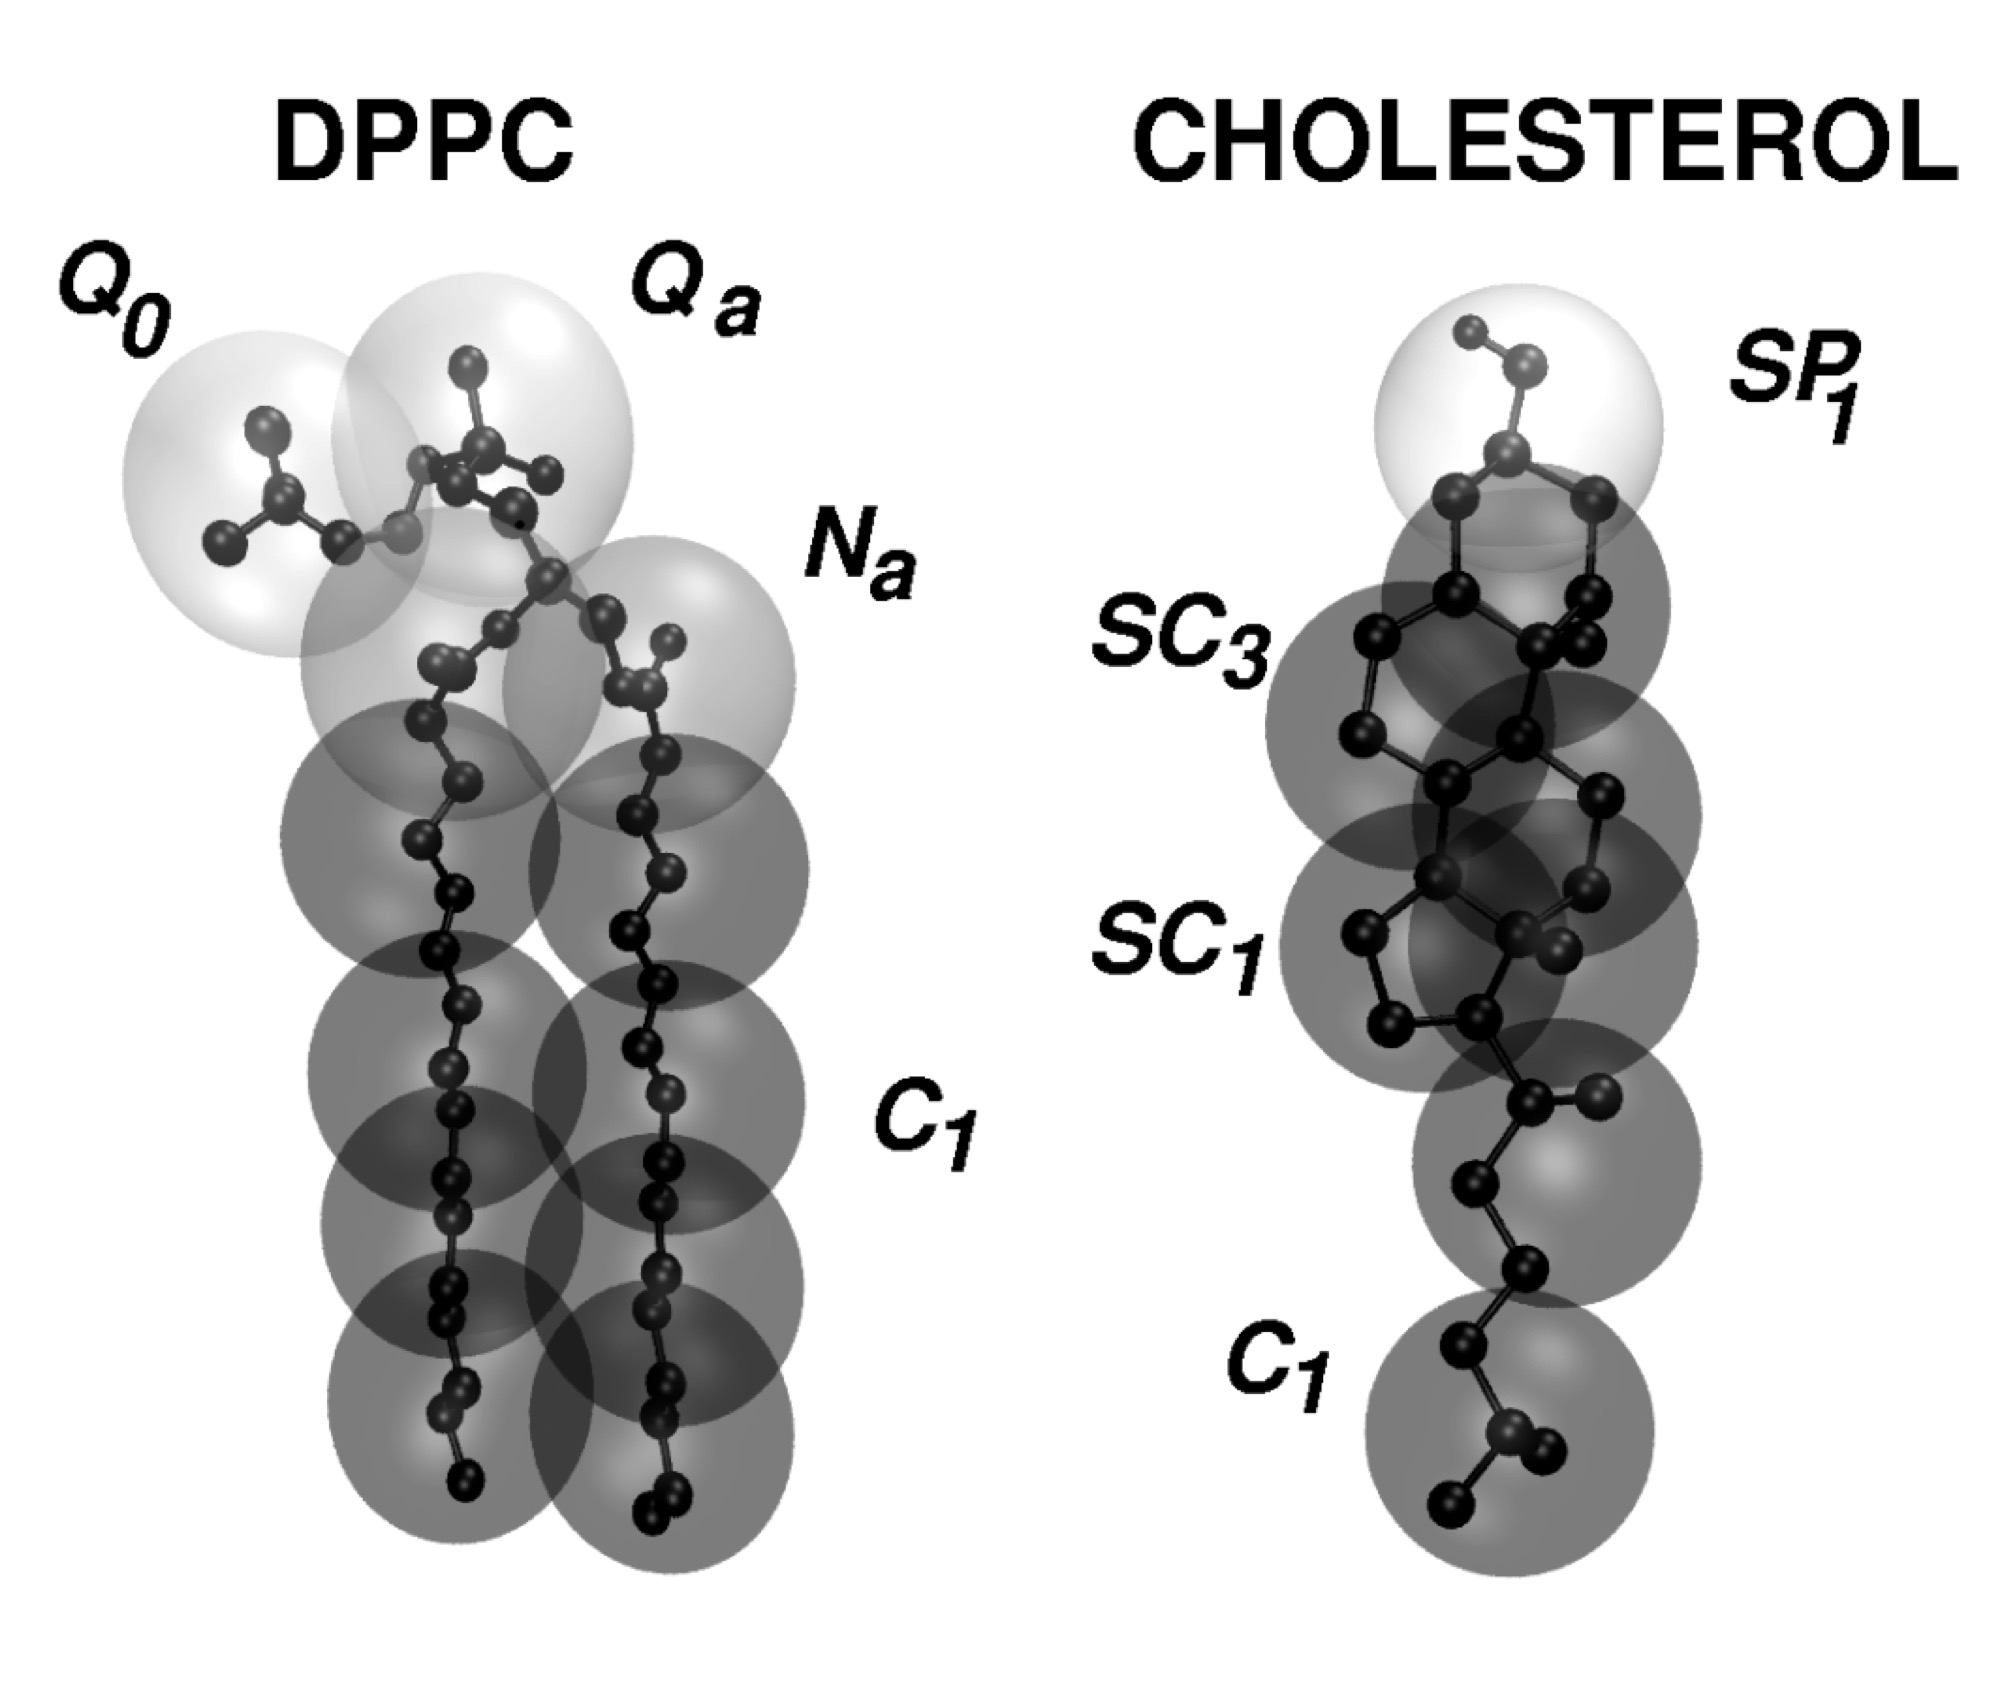
\includegraphics[width=0.4\linewidth, align=c]{2methods/pics/martini_lipids.jpg} \label{fig:martini_lip}}
\subbottom[]{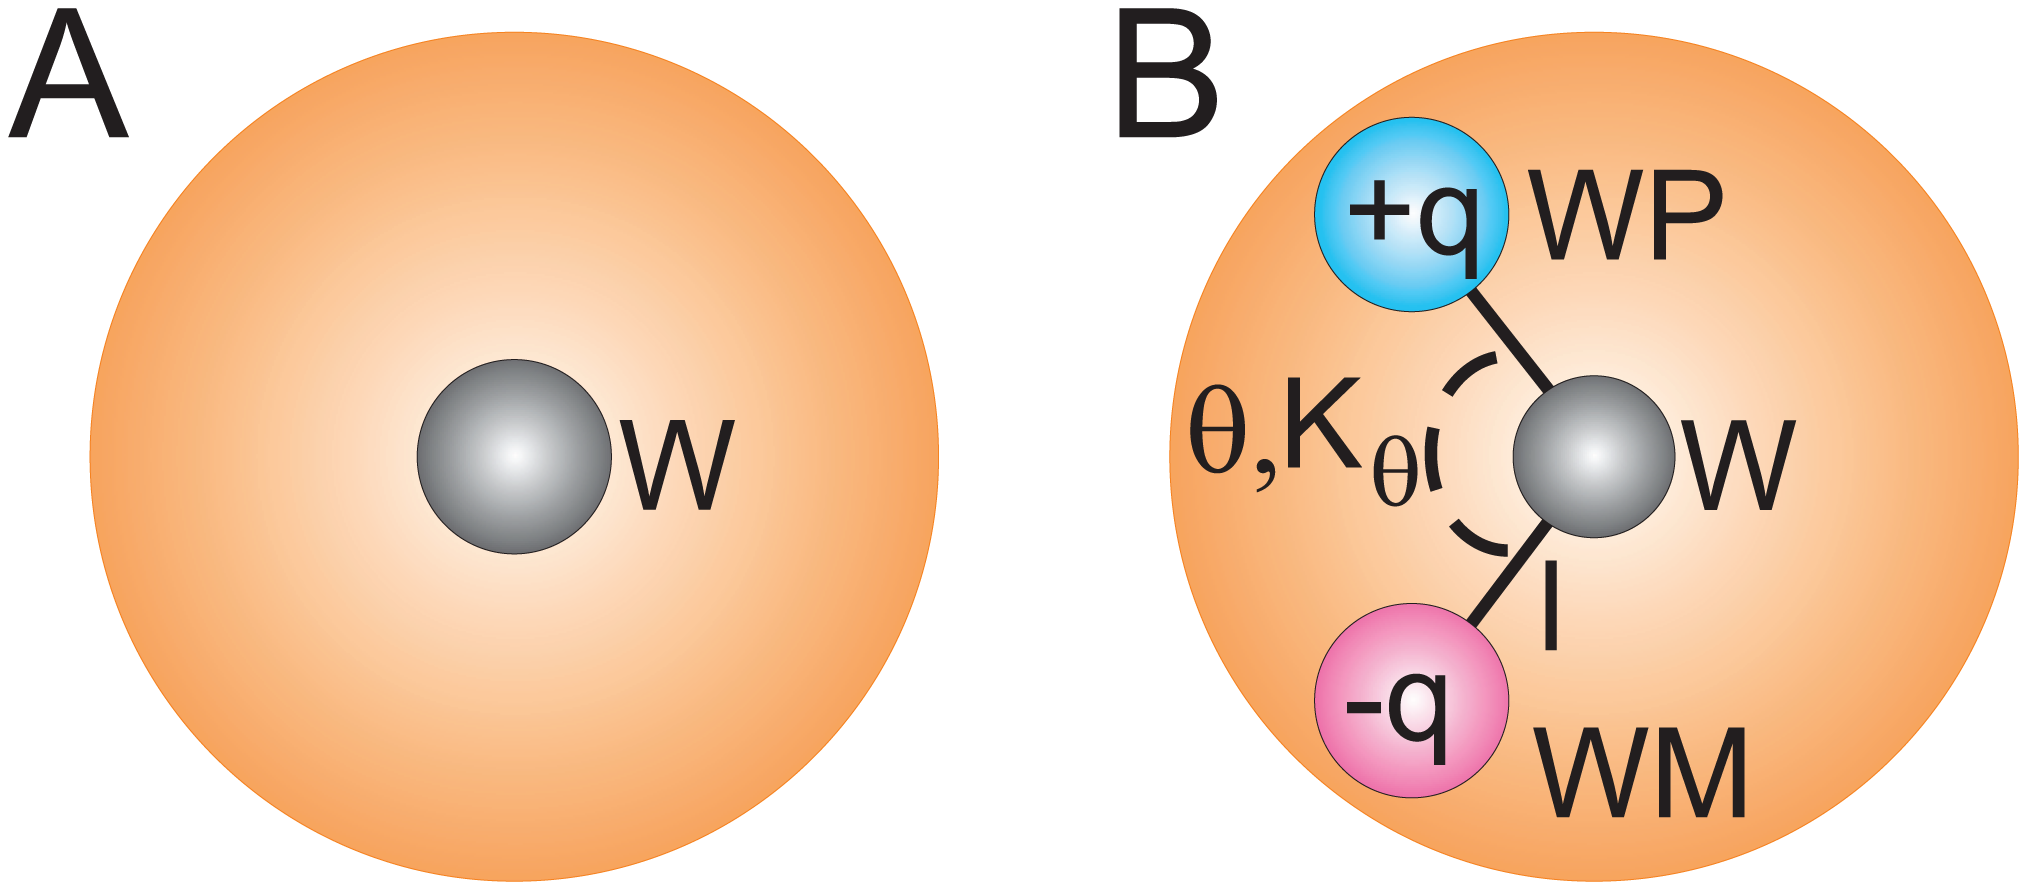
\includegraphics[width=0.35\linewidth, align=c]{2methods/pics/martini_polar.png} \label{fig:martini_w}}
%
\caption[MARTINI force field mapping for amino acids, lipids and water]{Description of amino acids (a), example lipids (b) and water models (c) in the MARTINI force field. In (c) the orange sphere represents the van der Waals radius of the central atom. Reproduced from \citet{Monticelli2008,calgary_site,Yesylevskyy2010}}
\label{fig:martini}
\end{figure}
%
Overall, the MARTINI force field pushes the limits of simplification to enhance the simulations speed-up, with considerable gain in efficiency with respect to atomistic or even SIRAH simulations. Despite it can not capture some fine details of the systems studied, it has been successfully applied to describe the behaviour of many biological membranes \citep{Khalid2019,Samsudin2017}, lipid self-assembly \citep{Marrink2007} and peptide-membrane binding \citep{Song2019}. The (re)introduction of a more detailed water model allowed the description of electroporation processes and the translocation of ions through bilayers \citep{Yesylevskyy2010}.

\subsection{Backmapping techniques} Coarse-grained descriptions are very effective in reproducing long time scales; however, to retrieve finer details after such extensive exploration, backmapping techniques have been designed to obtain atomistic configurations from the coarse-grained ones \citep{Wassenaar2015}. These backmapped structures can in turn be simulated at the atomistic level to explore the short time scale movements around such interesting conformation. The easy conversion between the two resolution, gave rise to many multiscale studies applied to biomolecular systems \citep{Lee2012}.

\section{Validation and challenges of MD simulations}

Validation of MD simulations is performed by comparison with experiments: the same properties obtained experimentally are computed from the MD trajectory as well, and the two compared. If these are correctly reproduced, it is usually assumed that the simulation is sampling the correct ensemble of states and then one can identify in the simulation the determinants responsible for the experimental outcome of interest, which are not accessible by the experiment itself.

The comparison however is not always easy: often the experimentally measured quantity is an average in time and/or space (for example Circular Dichroism spectra or SAXS profiles of a peptide in solution) and many different combinations of computationally derived structure ensembles can produce compatible results. It is still challenging to compare experimentally derived ensembles and the ones derived by molecular simulations. Indeed the extracted average properties may be different, so it is important to understand which are the relevant ones playing a role in the measured ensemble before attempting comparisons.

Thus, in the validation of MD outcomes, it is important to have a critical attitude and to interpret the result within the validity of the approximation \citep{VanGunsteren2008}.
%
Indeed, agreement may arise from either a simulation that reflects correctly the experimental system; but also when the property examined is insensitive to the details of the simulated trajectory, or it can be a result of compensation of errors, which is more likely to  occur for systems with a high number of degrees of freedom.
%
Similarly, disagreement may hint at an error in the simulation (either in the model, the implementation, or simply the estimated simulation's convergence) or an error in the interpretation and/or conditions of experimental set-up (either in the result itself o its interpretation), so that both must be carefully checked to improve a convergence in the agreement.
%
Some apparently negative results may suggest or stimulate new experimental settings to validate the hypotheses one was set to test \citep{Goncalves2013,Meissner2014}.

Additionally, simulations still suffer from the limited computational time available: most of the times, the real experimental system is simply too large to be reproduced and the time scale of the process too long. Simulations are thus confined to explore a restricted space, implying that the initial conditions must be chosen carefully to optimise the search and avoid any bias which might persist for the whole length of the simulation. The use of enhanced MD techniques can increase the chances of sampling relevant states \citep{Bernardi2015}.
%
As a non comprehensive list of these techniques, we mention replica-exchange algorithms \citep{Best2005} which combine together multiple simulations held at different conditions; local potential-energy elevation (or metadynamics) \citep{Barducci2010,Barducci2011} which avoids the re-sampling of already visited conformations adding an energy penalty to them; umbrella sampling \citep{Mills2008} which reconstructs free-energy barriers from simulations performed at specific values of the coordinate along which the barrier exists; or finally the simple use of higher temperature to overcome energy barriers \citep{Kirkpatrick1983}.

Finally, one should keep in mind that the force fields used are far from optimal, partly because they rely on approximate functional forms, and partly because it is difficult to find experimental observables measured with the desired resolution able to discriminate between sets of parameters.

Nevertheless, it remains important to note the contribution that Molecular Dynamics simulations have played in disclosing important details behind biophysical processes and in unravelling molecular details not accessible to experiments.
% cite rev


\section{MD simulations: successes} \label{sec:md_lit}
Consistently with the focus of this thesis, we will privilege examples of simulations investigating antimicrobial peptides as well as self-assembling ones, showing how computational techniques can help the design of novel molecules with improved specific characteristics.

\subsection{Simulations of antimicrobial peptides}
MD simulations of antimicrobial peptides are quite well documented since the first developments of the technique. Such peptides are a suitable system for a computational investigation as, in most of the cases, their mechanisms of action are not completely understood from the experimental information available (see Section \ref{AMP_mechs}). As experiments prove that even the mutation of one single residue in short AMPs can change remarkably the antimicrobial activity of the sequence (see Section \ref{sec:amp_design}), it is then clear that their action is governed by subtle atomic interactions, so that MD simulations, with their atomistic resolution, can help understanding this aspect.

\paragraph{Systems} As mentioned in the previous chapter, it has been proposed that most AMPs act through a process of attraction to the bacterial membrane, possible aggregation with other copies of the same sequence, insertion, and membrane lysis. The time scales of the overall process (at least of the order of microseconds and up to seconds) are accessible using coarse-grained techniques, but not - or rarely - atomistic ones.
%
For this level of description instead, the different steps are usually investigated separately, based on prior hypotheses: for example, the peptide can be positioned close to the membrane surface \citep{Wang2012}, or placed directly within the membrane core with different insertion depths to verify which configurations are the most disruptive ones \citep{Lipkin2017}. The full insertion process will be then reconstructed from a ``stepwise" knowledge combining the different states sampled.
%
For these reasons, the choice of the conformation to simulate, i.e.\ the initial conditions in terms of the mutual position of peptide and membrane, is crucial, as it likely biases the simulation towards the sampling of a particular subset of configurations. Recent advances in the computational power are making possible the simulations of the full process even at the atomistic resolution for simple enough systems \citep{Ulmschneider2017,Sun2015}, nevertheless the ``stepwise" approach is still common and the preferred one in case of complex AMP systems.

\paragraph{Model membranes} The second important choice in the setup of a simulations of antimicrobial peptides concerns the model of the membrane to simulate. In an effort to keep complexity low, bacterial and mammal membranes are often modelled with a minimal number of lipids.
%
Usually, models of bacterial membrane retain as only key characteristic an overall negative charge, with about 25\% of anionic lipids ($-1\,e$ charge) \citep{Lipkin2017,Wang2012,Zhao2018,Chen2019}.
For a model mammal membrane instead, only zwitterionic lipids are employed, with the occasional inclusion of cholesterol, as it is deemed important in describing more realistically their behaviour \citep{Lipkin2017,Wang2012,Zhao2018,Chen2019,Risselada2008}.
Because of their simplicity, these systems are used in experiments \citep{Castelletto2016,Tang2009,Glukhov2005}, making possible a direct comparison with simulations.
Therefore, even if these simple membranes do not model accurately the structure of the cellular envelope, simulations and experiments of these systems provide a first explanation of some steps of the antimicrobial activity, with the two techniques complementing and validating each other.

Nevertheless, attempts to model cell membranes more accurately have been pursued. This can be performed at the atomistic level \citep{Piggot2011}
but the task is especially suited for a coarse-grained description, as the inclusion of all the elements of the cell membranes results in quite large systems for which atomistic computations started only in recent years to be affordable.
%
Accordingly, coarse-grained (MARTINI) simulations have been incorporating more and more components into model membranes, describing the bacterial inner membrane, the bacterial wall, and finally the combination of the two \citep{Khalid2019} (see Figure \ref{fig:ff}, bottom).
%
These large scale, coarse-grained simulations provide information on the mechanic characteristics of the system: for example, simulation of the outer membranes of Gram-negative bacteria combined with the peptidoglycan layer (which, in bacteria, is positioned between the two membranes) elucidated how the distance between the two is variable, thanks to the presence of Braun's lipoproteins \citep{Asmar2018} which act as a bridge between them, and can bring them closer by bending and tilting.
%
On the other hand, the permeability of membranes to ions and small compounds needs to be assessed at the atomistic level, and to access informative simulation time scales, smaller and simpler systems must be chosen for the task (e.g.\ the inner membrane only), often together with enhanced MD techniques such as metadynamics, umbrella sampling, and replica exchange umbrella sampling. \citep{Sun2016,Piggot2011,Carpenter2016,Pokhrel2018}.

\paragraph{Force field comparison} Finally, simulations of the peptide interaction with a model membrane are clearly determined by the parametrisation of the force field employed for protein and lipids (and by their mutual consistency).
%
There are multiple evidence suggesting that different force fields produce very different outcomes when simulating the same system, under the same conditions \citep{Wang2014,Bennett2016,Sandoval-Perez2017}. This is also valid for simulations of pure lipid patches (see Chapter \ref{chapter:lip_par}), resulting in incompatible values of area per lipid, organisation of the tails and energetic profiles across the membrane, and thus has an impact in the simulations of AMPs interacting with a membrane.

For example \citet{Wang2014} observed significantly different levels of unfolding for the AMP melittin within a model membrane at the change of the force field, namely CHARMM27 and 36 (for protein and lipids respectively) \citep{MacKerell1998,Klauda2010}, OPLS all atoms (for protein) and united atoms (for lipids) \citep{Jorgensen1996} and GROMOS 53A6 \citep{Oostenbrink2004}; while \citet{Bennett2016} proved that the propensity of the synthetic AMP CM15 to form pores strongly depends on the force field used but also on some extent - at least at the time of the work - on the MD engine used (GROMACS compared to NAMD \citep{Phillips2005}).

A more systematic investigation was performed by \citet{Sandoval-Perez2017}, who focussed on the reproduction of membrane-protein interactions (in GROMOS 54A7 \citep{Schmid2011}, CHARMM36, Amber14SB/Slipids \citep{Jambeck2012} and Amber14SB/Lipid14 \citep{Dickson2014}).
%
While all of the force fields were able to reproduce the overall positioning of transmembrane proteins in the case studies tested, they showed discrepancies for amino acid side chains insertion depth and energy.
%
Interestingly, all parametrisations gave a very broad minimum for the insertion position of Tryptophan, in line with the different roles this amino acid is supposed to assume: either an anchoring point positioned deeper in the hyrophobic region, or a partner for hydrogen bonding with the hydrophilic heads \citep{Chan2006}.

The subtle differences between parametrisations lead to the conclusion that for every particular system tested, the comparison with at least one experimentally measured quantity would be the only way to assess the simulations performance accurately.

\paragraph{Simulations of membrane-peptide interaction: examples} Even in the context of a simplified scenario and with the caveats coming from the parametrisation chosen, simulations of antibacterial peptides on a membrane have been successful in elucidating some AMPs mechanisms.
%
The first important contribution consists in the introduction of the disordered toroidal pore concept: as explained in the previous chapter (Section \ref{AMP_mechs}), the models of membrane poration due to AMPs consist often in ordered structures where many peptides gather together to contour a pore (see Figure \ref{fig:amp}), and they are either in contact with the hydrophobic tails of the lipids (barrel-stave model), or with their head, as lipid molecules bend around the pore to keep their tails screened from the outside environment (toroidal pore model). However, simulations of the short helical peptide magainin MG-H2 \citep{Leontiadou2006}, among others, showed that a single copy of the helix inserted at an angle with the normal to the membrane plane, and was sufficient to displace the lipids around in a non organised manner, and form a water-filled pore (Figure \ref{fig:dis_pore}).
%
\begin{figure}[t!]
\centering
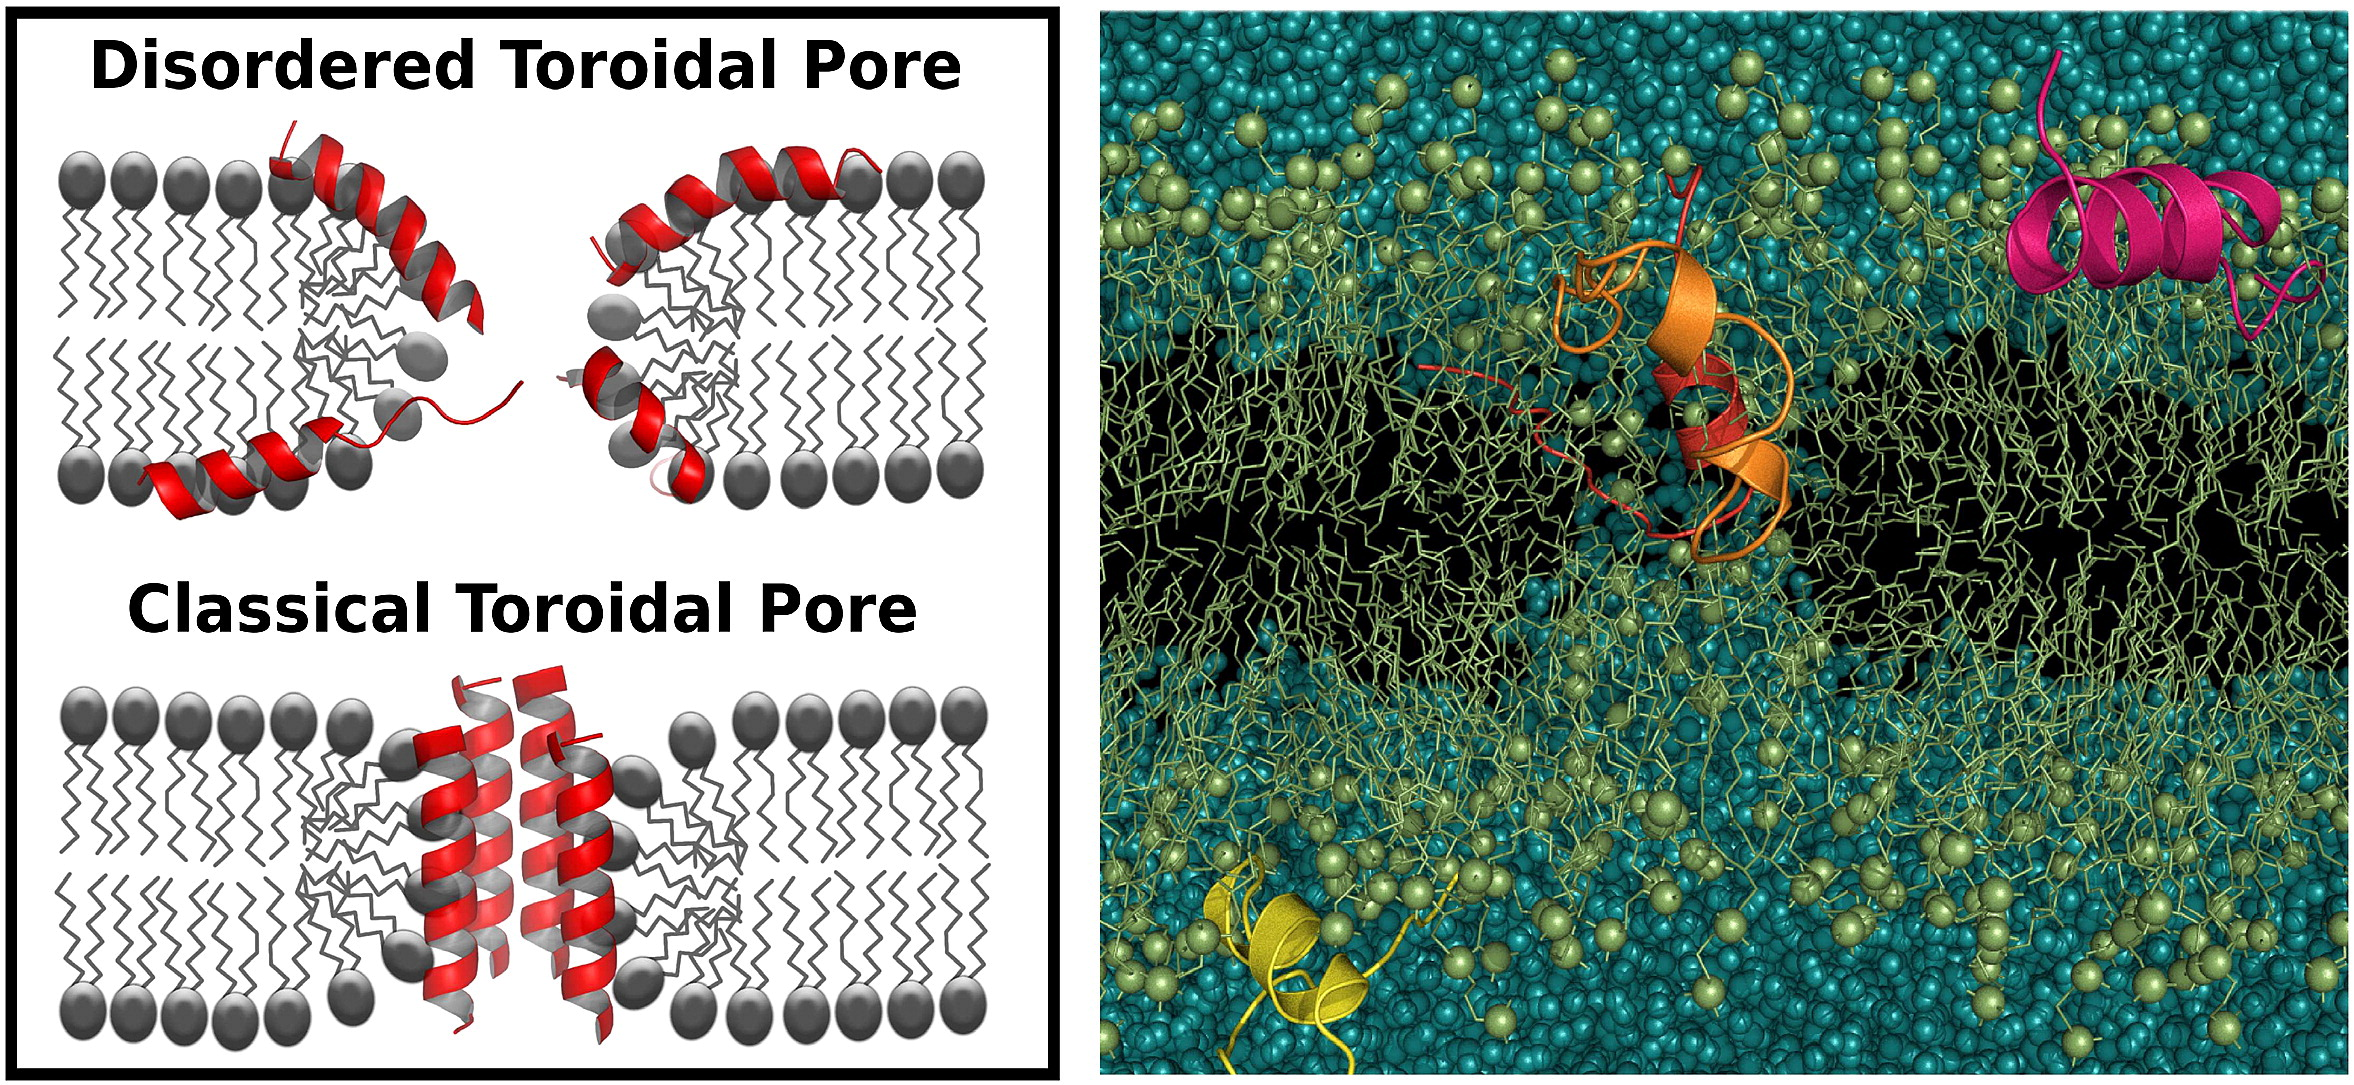
\includegraphics[width=0.8\linewidth]{2methods/pics/disordered_pore.jpg}
%
\caption[Disordered pore model]{(Left) A cartoon image comparing the disordered toroidal pore state (lack of a well defined peptide orientation) to the traditional view. (Right) A snapshot of the disordered toroidal pore from simulations of melittin in DPPC. Peptides in cartoon, lipids in lines, water and ions in bead representation. Reproduced from \citet{Sengupta2008}.}
\label{fig:dis_pore}
\end{figure}

% INITIAL CONDITION: SECONDARY STRUCTURE - KEPT/LOST
Regarding possible rearrangements of the antimicrobial peptide structure when interacting with a membrane, simulations of cathelicidin LL-37 on pure POPG (anionic) and POPC (zwitterionic) lipid patches showed that LL-37 has a propensity to bind to the former, as expected due to the opposite charge that membrane has with respect to the cationic peptide \citep{Zhao2018}. However the simulations highlighted also that, in contact with POPC, the helical secondary structure was lost, while the interaction with POPG preserved it, suggesting that the spatial arrangement of the residues, and not only the overall chemical character, is important for their action. Such type of information is hardly available to experiments or through a theoretical reasoning.

% INITIAL CONDITION - NO PRE-INSERTED PEPTIDE, SEE FULL TRANSLOCATION
The improvements in computational resources is slowly pushing the extent of simulation time to the microsecond time scale.
%
Thus in a recent example, the translocation of the helical PGLa peptide through the membrane has been observed as a rare event dependent on the concentration of the peptide. This event happened on the multi microsecond time scale without the formation of an organised pore \citep{Ulmschneider2017}. The \emph{in silico} experiment still benefited of an enhanced sampling in the form of a higher temperature as simulations were run at 363 K (rather than the usual 303 K), but no pre-insertion of the peptide was performed. This study shed light on a possible mechanism of permeabilisation which is usually overlooked in favour of processes involving organised channels and pores. 

% INITIAL CONDITION - NO PRE-INSERTED PEPTIDE, EXPLAIN POLYARGININES
Similarly, simulations were able to shed light on the mechanism of translocation of Arginine-rich peptides 
\citep{Sun2015}. These sequences have high positive charge, but despite this, possess a high propensity to penetrate membranes, overcoming the hydrophobic region represented by the lipid tails. Very similar peptides where the Arginines were swapped with Lysines showed no significant penetration.
%
A commonly used explanation considers polyarginine translocation a quasi-equilibrium process, but this does not explain the selectivity against Lysines rich peptides.
%
After extensive simulations of the two systems (multiple, hundreds of nanosecond long runs), the proposed mechanism involves the spontaneous formation of pores initiated by random (thermal) fluctuations of the position of the lipids: in some of these rare events, the transient pore would be occupied by a peptide (a precursor), which slows down the pore closure. In such situation, the translocation of other copies of the peptide is highly favoured (if their concentration is sufficiently high) as they aggregate with the precursor inside the membrane and are then pushed toward the opposite side where there is a lower charge density.
%
Differently from polyarginines, polylysines have a much lower aggregation propensity, so that the presence of a precursor peptide inside the membrane does not induce an enhanced insertion of further peptides.
%
\begin{figure}[t!]
\centering
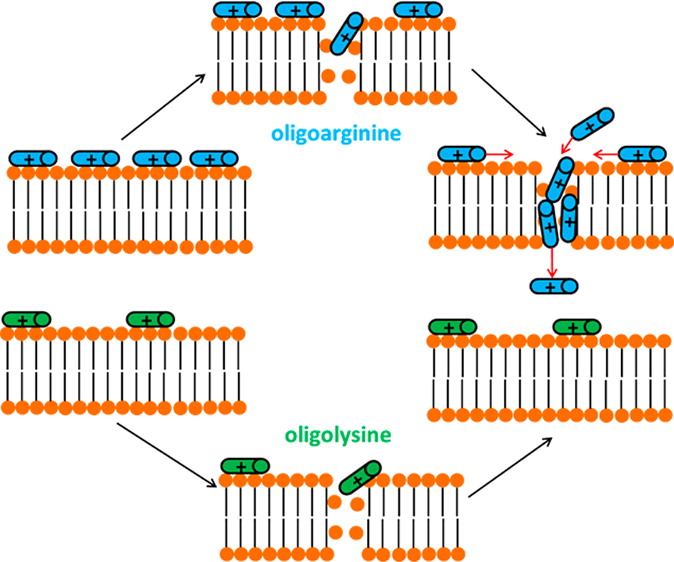
\includegraphics[width=0.65\linewidth]{2methods/pics/polyarg.jpeg}
%
\caption[Polyarginine translocation]{Cartoon representation of the different assembly mechanism that allow polyarginines but not polylysines to translocate through spontaneously formed pores. Reproduced from \citet{Sun2015}.}
\label{fig:polyArg}
\end{figure}

% OLIGOMERISATION
The last example brings the attention on whether oligomerisation is necessary for an efficient antimicrobial activity. Contrary to oligomerisation in solution, which can happen on shorter time scales, the spontaneous aggregation of peptides on a membrane surface requires a long time, as the structures must diffuse on the membrane to meet each other, and many other competing processes (such as insertion) are happening at the same time. MD simulations offer insights on this aspect as well.

% OLIGOMERISATION - NO BIASED SAMPLING
In a recent example, simulations of maculatin (an helical AMP) showed that the pores it forms can include a variable number of helices and thus assume many different conformations \citep{Wang2016}. The suggested process of pore formation proceeds via insertion of a single residue, closely followed by other ones which are able to penetrate the membrane thanks to the lipid defects already created by the first peptide.

% OTHER NON AMP EXAMPLES
Similar investigations were carried on also for other aggregating cell penetrating peptides, which are not antimicrobial: as such, some of them aim at inserting within cells without necessarily causing poration. One example is constituted by the influenza fusion peptides, which have been extensively studied with a simulation set up similar to the one mentioned for AMPs: a few copies of the peptide positioned on a model membrane oligomerised into aggregates of different sizes and inserted into the membrane, perturbing its local curvature \citep{Haria2014,Collu2015}.

% OLIGOMERISATION - PRE-ASSEMBLED
To be noticed that, when investigating oligomerisation, the size of the system must necessarily be increased to include all the copies necessary to form the aggregates observed experimentally. As such, with the present accessible computer time, not all the systems can be investigated from unbiased initial conditions.
%
In the case of protegrin, a $\beta$-hairpin antimicrobial peptide which has been long though to act through the formation of transmembrane $\beta$-barrels, many variables can influence the outcome of the unknown final structure.
%
To overcome such problems, a semi-systematic investigation has been carried on by \citet{Lipkin2017}, simulating different assembly (see Figure \ref{fig:ff}, top).
%
Microsecond long simulations discriminated which ones of these initial configuration formed stable pores for the whole length of the simulations, and the ones which were disrupted. As in the previous example, several different possibilities were found stable in solution, suggesting that single AMPs might have multiple mechanisms of insertion into membranes.

Most of the examples above employ atomistic descriptions of the system, but similar investigations have been carried on also using the MARTINI force field. %, indeed the coarse-grained description does capture the pore-forming behaviour of some AMPs.
%
As an example, MARTINI simulations of maculatin and aurein on POPC membranes showed different propensities for pore formation versus aggregation, showing that the coarse-grained model retains enough details and chemical information to reproduce different membrane-perturbing behaviours \citep{Balatti2017}.
%
Nevertheless, the developers of the MARTINI model themselves pointed out how some aspects of pore formation might not be captured in a satisfactory way \citep{Marrink2013}. For example the penetration of water can be misrepresented, as can be expected from a model which clusters four water molecules together (indeed some pore conformations allow for the passage of fewer water molecule, if not one, at the time). As such, the MARTINI membranes can be overstabilised, and have less propensity to break and porate, with respect to their real counterpart.

In general, the outlook of simulations of antimicrobial peptides interacting with membranes goes in the direction of reproducing longer time scales thanks to the enhanced computational power available. %, trying to match the experimental findings showing that many antimicrobial related processes happen at the microsecond scale or beyond.
%
This enhanced power would also reduce the need to use biased initial conditions or higher temperatures to speed up the simulations.
%
Moreover, gathering the contribution of the whole community, simulations will likely go in the direction of modelling more accurately the bacterial membrane (see previous paragraph). %, and while this is already at an advanced stage for coarse-grained simulations, it is still an ongoing process for atomistic ones.
%
Finally, the force field issue must be solved in collaboration with experimentalists, finding new tests and experimental quantities to compare the computational outcome with, and make the different parameters sets converge toward a similar description of the phenomena observed, which is consistent with the experimental results.


\paragraph{Simulation-aided AMPs design} \label{sec:design_md_examples}

The role of simulations in aiding AMPs design has been briefly sketched in Section \ref{sec:amp_design}. As pointed out, MD simulations are hardly a tool to analyse large dataset, therefore %a systematic analysis can be performed for very small systems only, or, alternatively,
the investigation focuses on a few selected sequences.

Simulations can be helpful in integrating structural information which is otherwise lacking: such approach was followed by \citet{Liu2018} to complement the chemical features available on a dataset of short AMPs, and the overall information was used to feed a predictor of AM activity of novel sequences. Preliminary results showed that this improved significantly the ability of the predictor to discriminate whether a new sequence was suitable for antimicrobial activity or not.

Another commonly followed approach consists in using simulations to elucidate the reasons why a particular mutation is effective in terms of increased activity or decreased toxicity. Mutation screenings can be afforded experimentally on short sequences, but they are usually limited to single point mutations, as testing all the possible combined mutations is prohibitive. However, once assessed the importance of a given substitution, it is interesting to understand the mechanism behind it.
%
For example, simulations of ovispirin and a mutant peptide with reduced toxicity showed that the bend of the helix in the latter was responsible for mitigating the interaction with mammal membranes and thus reducing haemolysis \citep{Khandelia2005}.
%
In another example, temporin and a derived sequence with improved activity were investigated. Simulations showed that the mutant had a reduced aggregation propensity in water, so that more copies were ready to bind to the membrane and thus disrupt it \citep{Farrotti2017}.

In general, the protocol of integrating simulations and design is usually customised according to the system in exam, as the field has not reached yet a systematic organisation.
%
However, it is clear that simulations used in conjunction with experimental testing can be used to optimise already available AMP sequences, and thus contribute to device design rules for the creation of synthetic peptides with tailored properties.


\subsection{Simulations of self-assembling peptides}
Self-assembling peptides are another fascinating and challenging topic that MD simulations can help investigating. Simulating such systems implies different challenges with respect to the ones faced when simulating AMPs on membranes \citep{Frederix2018,Orsi2018}.

In theory, the set up of the system is quite straightforward: only the solvent characteristics and optionally the experimental salt concentration need to be matched, then choosing a random initial configuration of the molecules - in the desired concentration - would allow the simulation of the process of interest.
%
In reality, to reproduce the dilution employed in experiments, a considerable volume needs to be simulated to host enough copies of the peptide to observe the assembly of large enough oligomers.
%
With this approach, the time scale useful to witness a spontaneous assembly would greatly exceed the computational time available. For that reason, two main strategies have been adopted to follow assembly processes: coarse-grained simulations and/or  the  use  of pre-assembled structures. In the following we give a few examples of these two strategies. Other routes include the choice of an implicit solvent model \citep{Jusufi2013,Spaeth2011}, or the use of a Monte Carlo sampling which can sometimes be less time consuming as it does not evolve the system through dynamics, but generates new configurations at random and accepts the ones energetically favoured \citep{He2001,Majumdar2019,Luo2015}. 

Many studies have been performed with the coarse-grained MARTINI force field to witness assembly of surfactants \citep{Wu2012}, polymers \citep{Wang2012poly,Bochicchio2017}, lipids \citep{Lee2011,Brocos2012} or peptides \citep{Guo2012,Seo2012}.
%
Regarding the latter, the assembly in water of peptide amphiphiles (PAs) into cylindrical fibers has been simulated \citep{Lee2012}, showing a transition from small micelles to long fibres (Figure \ref{fig:PA}). This example of minimal PA structures is particularly interesting for the study of AMPs as well, as it shares with them the amphiphatic character, so that having a general knowledge on how AMP analogous sequences assemble together would help in tuning their aggregation properties in water prior to the delivery to the membrane.
%
\begin{figure}[t!]
\centering
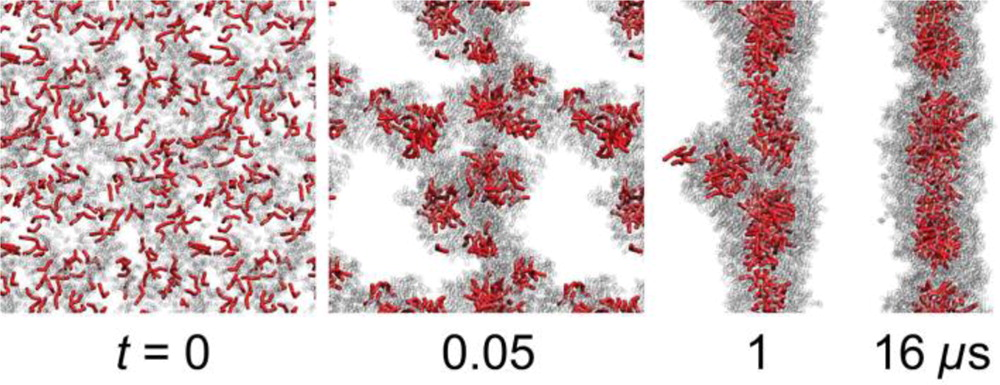
\includegraphics[width=0.8\linewidth]{2methods/pics/PA.jpeg}
%
\caption[Peptide amphiphiles assembly through MARTINI simulations]{Process of peptide amphiphiles (PA) fiber formation assessed through MARTINI simulations. Hydrophobic tails in red, peptides in gray. Reproduced from \citet{Lee2012}.}
\label{fig:PA}
\end{figure}

The second approach consists in preparing the system in pre-assemble states that are somewhat suggested by experimental evidences, and further to this using MD simulations to verify whether the conformations are kept or disrupted, and which one is the one most energetically favoured. 
%
In the work mentioned about peptide amphiphiles \citep{Lee2012}, pre-assembled fibres have been simulated at the atomistic level, to confirm the stability of the structures found with a coarse-grained approach.

The same approach has been widely employed also in cases where the final assembly was hypothesised to have a high degree of order, achievable only with a long sampling \citep{Gudlur2012}.

Similar procedures have been crucial in elucidating the assembly process of viral capsids. Capsids are very large systems and the assembly of their protein subunits is mediated by energy barriers. For these reasons, pre-assembled systems have been simulated to understand the interaction between the components and thus the first mechanisms of the assembly. This has been done recurring to ultra coarse-grained or elastic network models \citep{Grime2016,AbiMansour2014} first, and only in the most recent computational advances to atomistic simulations \citep{Perilla2016,Hadden2018,AbiMansour2014}.


\paragraph{}
The examples above show how Molecular Dynamics simulations have been employed for the investigation of many different systems, adapting the resolution, set up and the techniques related to better query the systems of interest. Such overview suggests then that simulations would be a suitable tool to investigate the system of interest of this work, namely the self-assembling antimicrobial peptide capzip. The two aspects of its behaviour will be studied separately, adopting the necessary approximations and strategies to make the simulations efficient and to query the related questions at each time.

The details of the systems simulated and the specific parameters used for each case can be found in the relative sections of the following chapters, together with an extensive explanation of the motivation of the choices made.
